% Options for packages loaded elsewhere
\PassOptionsToPackage{unicode}{hyperref}
\PassOptionsToPackage{hyphens}{url}
%
\documentclass[
  letterpaper,
  oneside,
  open=any]{scrbook}

\usepackage{amsmath,amssymb}
\usepackage{iftex}
\ifPDFTeX
  \usepackage[T1]{fontenc}
  \usepackage[utf8]{inputenc}
  \usepackage{textcomp} % provide euro and other symbols
\else % if luatex or xetex
  \usepackage{unicode-math}
  \defaultfontfeatures{Scale=MatchLowercase}
  \defaultfontfeatures[\rmfamily]{Ligatures=TeX,Scale=1}
\fi
\usepackage{lmodern}
\ifPDFTeX\else  
    % xetex/luatex font selection
\fi
% Use upquote if available, for straight quotes in verbatim environments
\IfFileExists{upquote.sty}{\usepackage{upquote}}{}
\IfFileExists{microtype.sty}{% use microtype if available
  \usepackage[]{microtype}
  \UseMicrotypeSet[protrusion]{basicmath} % disable protrusion for tt fonts
}{}
\makeatletter
\@ifundefined{KOMAClassName}{% if non-KOMA class
  \IfFileExists{parskip.sty}{%
    \usepackage{parskip}
  }{% else
    \setlength{\parindent}{0pt}
    \setlength{\parskip}{6pt plus 2pt minus 1pt}}
}{% if KOMA class
  \KOMAoptions{parskip=half}}
\makeatother
\usepackage{xcolor}
\setlength{\emergencystretch}{3em} % prevent overfull lines
\setcounter{secnumdepth}{5}
% Make \paragraph and \subparagraph free-standing
\ifx\paragraph\undefined\else
  \let\oldparagraph\paragraph
  \renewcommand{\paragraph}[1]{\oldparagraph{#1}\mbox{}}
\fi
\ifx\subparagraph\undefined\else
  \let\oldsubparagraph\subparagraph
  \renewcommand{\subparagraph}[1]{\oldsubparagraph{#1}\mbox{}}
\fi
\usepackage{color}
\usepackage{fancyvrb}
\newcommand{\VerbBar}{|}
\newcommand{\VERB}{\Verb[commandchars=\\\{\}]}
\DefineVerbatimEnvironment{Highlighting}{Verbatim}{commandchars=\\\{\}}
% Add ',fontsize=\small' for more characters per line
\usepackage{framed}
\definecolor{shadecolor}{RGB}{241,243,245}
\newenvironment{Shaded}{\begin{snugshade}}{\end{snugshade}}
\newcommand{\AlertTok}[1]{\textcolor[rgb]{0.68,0.00,0.00}{#1}}
\newcommand{\AnnotationTok}[1]{\textcolor[rgb]{0.37,0.37,0.37}{#1}}
\newcommand{\AttributeTok}[1]{\textcolor[rgb]{0.40,0.45,0.13}{#1}}
\newcommand{\BaseNTok}[1]{\textcolor[rgb]{0.68,0.00,0.00}{#1}}
\newcommand{\BuiltInTok}[1]{\textcolor[rgb]{0.00,0.23,0.31}{#1}}
\newcommand{\CharTok}[1]{\textcolor[rgb]{0.13,0.47,0.30}{#1}}
\newcommand{\CommentTok}[1]{\textcolor[rgb]{0.37,0.37,0.37}{#1}}
\newcommand{\CommentVarTok}[1]{\textcolor[rgb]{0.37,0.37,0.37}{\textit{#1}}}
\newcommand{\ConstantTok}[1]{\textcolor[rgb]{0.56,0.35,0.01}{#1}}
\newcommand{\ControlFlowTok}[1]{\textcolor[rgb]{0.00,0.23,0.31}{#1}}
\newcommand{\DataTypeTok}[1]{\textcolor[rgb]{0.68,0.00,0.00}{#1}}
\newcommand{\DecValTok}[1]{\textcolor[rgb]{0.68,0.00,0.00}{#1}}
\newcommand{\DocumentationTok}[1]{\textcolor[rgb]{0.37,0.37,0.37}{\textit{#1}}}
\newcommand{\ErrorTok}[1]{\textcolor[rgb]{0.68,0.00,0.00}{#1}}
\newcommand{\ExtensionTok}[1]{\textcolor[rgb]{0.00,0.23,0.31}{#1}}
\newcommand{\FloatTok}[1]{\textcolor[rgb]{0.68,0.00,0.00}{#1}}
\newcommand{\FunctionTok}[1]{\textcolor[rgb]{0.28,0.35,0.67}{#1}}
\newcommand{\ImportTok}[1]{\textcolor[rgb]{0.00,0.46,0.62}{#1}}
\newcommand{\InformationTok}[1]{\textcolor[rgb]{0.37,0.37,0.37}{#1}}
\newcommand{\KeywordTok}[1]{\textcolor[rgb]{0.00,0.23,0.31}{#1}}
\newcommand{\NormalTok}[1]{\textcolor[rgb]{0.00,0.23,0.31}{#1}}
\newcommand{\OperatorTok}[1]{\textcolor[rgb]{0.37,0.37,0.37}{#1}}
\newcommand{\OtherTok}[1]{\textcolor[rgb]{0.00,0.23,0.31}{#1}}
\newcommand{\PreprocessorTok}[1]{\textcolor[rgb]{0.68,0.00,0.00}{#1}}
\newcommand{\RegionMarkerTok}[1]{\textcolor[rgb]{0.00,0.23,0.31}{#1}}
\newcommand{\SpecialCharTok}[1]{\textcolor[rgb]{0.37,0.37,0.37}{#1}}
\newcommand{\SpecialStringTok}[1]{\textcolor[rgb]{0.13,0.47,0.30}{#1}}
\newcommand{\StringTok}[1]{\textcolor[rgb]{0.13,0.47,0.30}{#1}}
\newcommand{\VariableTok}[1]{\textcolor[rgb]{0.07,0.07,0.07}{#1}}
\newcommand{\VerbatimStringTok}[1]{\textcolor[rgb]{0.13,0.47,0.30}{#1}}
\newcommand{\WarningTok}[1]{\textcolor[rgb]{0.37,0.37,0.37}{\textit{#1}}}

\providecommand{\tightlist}{%
  \setlength{\itemsep}{0pt}\setlength{\parskip}{0pt}}\usepackage{longtable,booktabs,array}
\usepackage{calc} % for calculating minipage widths
% Correct order of tables after \paragraph or \subparagraph
\usepackage{etoolbox}
\makeatletter
\patchcmd\longtable{\par}{\if@noskipsec\mbox{}\fi\par}{}{}
\makeatother
% Allow footnotes in longtable head/foot
\IfFileExists{footnotehyper.sty}{\usepackage{footnotehyper}}{\usepackage{footnote}}
\makesavenoteenv{longtable}
\usepackage{graphicx}
\makeatletter
\def\maxwidth{\ifdim\Gin@nat@width>\linewidth\linewidth\else\Gin@nat@width\fi}
\def\maxheight{\ifdim\Gin@nat@height>\textheight\textheight\else\Gin@nat@height\fi}
\makeatother
% Scale images if necessary, so that they will not overflow the page
% margins by default, and it is still possible to overwrite the defaults
% using explicit options in \includegraphics[width, height, ...]{}
\setkeys{Gin}{width=\maxwidth,height=\maxheight,keepaspectratio}
% Set default figure placement to htbp
\makeatletter
\def\fps@figure{htbp}
\makeatother
% definitions for citeproc citations
\NewDocumentCommand\citeproctext{}{}
\NewDocumentCommand\citeproc{mm}{%
  \begingroup\def\citeproctext{#2}\cite{#1}\endgroup}
\makeatletter
 % allow citations to break across lines
 \let\@cite@ofmt\@firstofone
 % avoid brackets around text for \cite:
 \def\@biblabel#1{}
 \def\@cite#1#2{{#1\if@tempswa , #2\fi}}
\makeatother
\newlength{\cslhangindent}
\setlength{\cslhangindent}{1.5em}
\newlength{\csllabelwidth}
\setlength{\csllabelwidth}{3em}
\newenvironment{CSLReferences}[2] % #1 hanging-indent, #2 entry-spacing
 {\begin{list}{}{%
  \setlength{\itemindent}{0pt}
  \setlength{\leftmargin}{0pt}
  \setlength{\parsep}{0pt}
  % turn on hanging indent if param 1 is 1
  \ifodd #1
   \setlength{\leftmargin}{\cslhangindent}
   \setlength{\itemindent}{-1\cslhangindent}
  \fi
  % set entry spacing
  \setlength{\itemsep}{#2\baselineskip}}}
 {\end{list}}
\usepackage{calc}
\newcommand{\CSLBlock}[1]{\hfill\break\parbox[t]{\linewidth}{\strut\ignorespaces#1\strut}}
\newcommand{\CSLLeftMargin}[1]{\parbox[t]{\csllabelwidth}{\strut#1\strut}}
\newcommand{\CSLRightInline}[1]{\parbox[t]{\linewidth - \csllabelwidth}{\strut#1\strut}}
\newcommand{\CSLIndent}[1]{\hspace{\cslhangindent}#1}

\usepackage[default]{opensans}
\fontseries{lc}\selectfont
\makeatletter
\@ifpackageloaded{bookmark}{}{\usepackage{bookmark}}
\makeatother
\makeatletter
\@ifpackageloaded{caption}{}{\usepackage{caption}}
\AtBeginDocument{%
\ifdefined\contentsname
  \renewcommand*\contentsname{Table of contents}
\else
  \newcommand\contentsname{Table of contents}
\fi
\ifdefined\listfigurename
  \renewcommand*\listfigurename{List of Figures}
\else
  \newcommand\listfigurename{List of Figures}
\fi
\ifdefined\listtablename
  \renewcommand*\listtablename{List of Tables}
\else
  \newcommand\listtablename{List of Tables}
\fi
\ifdefined\figurename
  \renewcommand*\figurename{Figure}
\else
  \newcommand\figurename{Figure}
\fi
\ifdefined\tablename
  \renewcommand*\tablename{Table}
\else
  \newcommand\tablename{Table}
\fi
}
\@ifpackageloaded{float}{}{\usepackage{float}}
\floatstyle{ruled}
\@ifundefined{c@chapter}{\newfloat{codelisting}{h}{lop}}{\newfloat{codelisting}{h}{lop}[chapter]}
\floatname{codelisting}{Listing}
\newcommand*\listoflistings{\listof{codelisting}{List of Listings}}
\makeatother
\makeatletter
\makeatother
\makeatletter
\@ifpackageloaded{caption}{}{\usepackage{caption}}
\@ifpackageloaded{subcaption}{}{\usepackage{subcaption}}
\makeatother

\usepackage{hyphenat}
\usepackage{ifthen}
\usepackage{calc}
\usepackage{calculator}

\usepackage{graphicx}
\usepackage{wallpaper}

\usepackage{geometry}

\usepackage{graphicx}
\usepackage{geometry}
\usepackage{afterpage}
\usepackage{tikz}
\usetikzlibrary{calc}
\usetikzlibrary{fadings}
\usepackage[pagecolor=none]{pagecolor}


% Set the titlepage font families







% Set the coverpage font families

\ifLuaTeX
  \usepackage{selnolig}  % disable illegal ligatures
\fi
\usepackage{bookmark}

\IfFileExists{xurl.sty}{\usepackage{xurl}}{} % add URL line breaks if available
\urlstyle{same} % disable monospaced font for URLs
\hypersetup{
  pdftitle={CPS Acoustic Classification},
  pdfauthor={Alice Beittel},
  hidelinks,
  pdfcreator={LaTeX via pandoc}}

\title{CPS Acoustic Classification}
\author{Alice Beittel}
\date{}

\begin{document}
%%%%% begin titlepage extension code

  \begin{frontmatter}

\begin{titlepage}
% This is a combination of Pandoc templating and LaTeX
% Pandoc templating https://pandoc.org/MANUAL.html#templates
% See the README for help

\thispagestyle{empty}

\newgeometry{top=-100in}

% Page color

\newcommand{\coverauthorstyle}[1]{{\fontsize{20}{24.0}\selectfont
#1}}

\begin{tikzpicture}[remember picture, overlay, inner sep=0pt, outer sep=0pt]

\tikzfading[name=fadeout, inner color=transparent!0,outer color=transparent!100]
\tikzfading[name=fadein, inner color=transparent!100,outer color=transparent!0]
\node[anchor=south west, rotate=0.0, opacity=1.0] at ($(current page.south west)+(0pt, 8.75in)$) {

\includegraphics[width=\paperwidth, keepaspectratio]{images/cover-header-2.png}};

% Title
\newcommand{\titlelocationleft}{2.3in}
\newcommand{\titlelocationbottom}{7in}
\newcommand{\titlealign}{left}

\begin{scope}{%
\fontsize{30}{36.0}\selectfont
\node[anchor=north
west, align=left, rotate=0] (Title1) at ($(current page.south west)+(\titlelocationleft,\titlelocationbottom)$)  [text width = 5in]  {\textcolor{black}{\bfseries{\nohyphens{CPS
Acoustic Classification}}}};
}
\end{scope}

% Author
\newcommand{\authorlocationleft}{2.3in}
\newcommand{\authorlocationbottom}{5in}
\newcommand{\authoralign}{left}

\begin{scope}
{%
\fontsize{20}{24.0}\selectfont
\node[anchor=north
west, align=left, rotate=0] (Author1) at ($(current page.south west)+(\authorlocationleft,\authorlocationbottom)$)  [text width = 5in]  {
\coverauthorstyle{Alice Beittel\\}};
}
\end{scope}

% Header
\newcommand{\headerlocationleft}{2.3in}
\newcommand{\headerlocationbottom}{9.8in}
\newcommand{\headerlocationalign}{left}

\begin{scope}
{%
\fontsize{16}{19.2}\selectfont
 \node[anchor=north west, align=left, rotate=0] (Header1) at %
($(current page.south west)+(\headerlocationleft,\headerlocationbottom)$)  [text width = 5in]  {\textcolor{white}{\nohyphens{NOAA
Technical Memorandum NMFS-XXX-\#\#}}};
}
\end{scope}

% Footer
\newcommand{\footerlocationleft}{6in}
\newcommand{\footerlocationbottom}{0.1\paperheight}
\newcommand{\footerlocationalign}{left}

\begin{scope}
{%
\fontsize{8}{9.6}\selectfont
 \node[anchor=north west, align=left, rotate=0] (Footer1) at %
($(current page.south west)+(\footerlocationleft,\footerlocationbottom)$)  [text width = 2.5in]  {{\nohyphens{U.S.
DEPARTMENT OF COMMERCE\\
\strut \\
National Oceanic and Atmospheric Administration\\
National Marine Fisheries Service\\
Northwest Fisheries Science Center}}};
}
\end{scope}

% Date
\newcommand{\datelocationleft}{6in}
\newcommand{\datelocationbottom}{2in}
\newcommand{\datelocationalign}{left}

\begin{scope}
{%
\fontsize{20}{24.0}\selectfont
 \node[anchor=north west, align=left, rotate=0] (Date1) at %
($(current page.south west)+(\datelocationleft,\datelocationbottom)$)  [text width = 2.5in]  {{\nohyphens{January
2023}}};
}
\end{scope}

\end{tikzpicture}
\clearpage
\restoregeometry
%%% TITLE PAGE START

% Set up alignment commands
%Page
\newcommand{\titlepagepagealign}{
\ifthenelse{\equal{left}{right}}{\raggedleft}{}
\ifthenelse{\equal{left}{center}}{\centering}{}
\ifthenelse{\equal{left}{left}}{\raggedright}{}
}
%% Titles
\newcommand{\titlepagetitlealign}{
\ifthenelse{\equal{left}{right}}{\raggedleft}{}
\ifthenelse{\equal{left}{center}}{\centering}{}
\ifthenelse{\equal{left}{left}}{\raggedright}{}
\ifthenelse{\equal{left}{spread}}{\makebox[\linewidth][s]}{}
}


\newcommand{\titleandsubtitle}{
% Title and subtitle
{\fontsize{30}{36.0}\selectfont
\textcolor{black}{\bfseries{\nohyphens{CPS Acoustic
Classification}}}\par
}%
}
\newcommand{\titlepagetitleblock}{
\titleandsubtitle
}

\newcommand{\authorstyle}[1]{{\fontsize{20}{24.0}\selectfont
#1}}

\newcommand{\affiliationstyle}[1]{{#1}}

\newcommand{\titlepageauthorblock}{
{\authorstyle{\nohyphens{Alice Beittel}{\textsuperscript{1}}}}}

\newcommand{\titlepageaffiliationblock}{
\hangindent=1em
\hangafter=1
{\affiliationstyle{
{1}.~NOAA Southwest Fisheres Science Center,~Southwest Fisheries Science
Center


\vspace{1\baselineskip} 
}}
}
\newcommand{\headerstyled}{%
{}
}
\newcommand{\footerstyled}{%
{}
}
\newcommand{\datestyled}{%
{}
}


\newcommand{\titlepageheaderblock}{\headerstyled}

\newcommand{\titlepagefooterblock}{
\footerstyled
}

\newcommand{\titlepagedateblock}{
\datestyled
}

%set up blocks so user can specify order
\newcommand{\titleblock}{{\titlepagetitlealign

{\titlepagetitleblock}
}

\vspace{4\baselineskip}
}

\newcommand{\authorblock}{{\titlepageauthorblock}

\vspace{2\baselineskip}
}

\newcommand{\affiliationblock}{{\titlepageaffiliationblock}

\vspace{2\baselineskip}
}

\newcommand{\logoblock}{}

\newcommand{\footerblock}{}

\newcommand{\dateblock}{}

\newcommand{\headerblock}{}
\newgeometry{top=3in,bottom=1in,right=1in,left=1.75in}
% background image
\newlength{\bgimagesize}
\setlength{\bgimagesize}{0.75\paperwidth}
\LENGTHDIVIDE{\bgimagesize}{\paperwidth}{\theRatio} % from calculator pkg
\ThisULCornerWallPaper{\theRatio}{images/corner-image.png}

\thispagestyle{empty} % no page numbers on titlepages


\newcommand{\vrulecode}{\rule{\vrulewidth}{\textheight}}
\newlength{\vrulewidth}
\setlength{\vrulewidth}{0pt}
\newlength{\B}
\setlength{\B}{\ifdim\vrulewidth > 0pt 0.05\textwidth\else 0pt\fi}
\newlength{\minipagewidth}
\ifthenelse{\equal{left}{left} \OR \equal{left}{right} }
{% True case
\setlength{\minipagewidth}{\textwidth - \vrulewidth - \B - 0.1\textwidth}
}{
\setlength{\minipagewidth}{\textwidth - 2\vrulewidth - 2\B - 0.1\textwidth}
}
\ifthenelse{\equal{left}{left} \OR \equal{left}{leftright}}
{% True case
\raggedleft % needed for the minipage to work
\vrulecode
\hspace{\B}
}{%
\raggedright % else it is right only and width is not 0
}
% [position of box][box height][inner position]{width}
% [s] means stretch out vertically; assuming there is a vfill
\begin{minipage}[b][\textheight][s]{\minipagewidth}
\titlepagepagealign
\headerblock

\titleblock

\authorblock

\affiliationblock

\vfill

\logoblock

\footerblock
\par

\end{minipage}\ifthenelse{\equal{left}{right} \OR \equal{left}{leftright} }{
\hspace{\B}
\vrulecode}{}
\clearpage
\restoregeometry
%%% TITLE PAGE END
\end{titlepage}
\setcounter{page}{1}
\end{frontmatter}

%%%%% end titlepage extension code

\renewcommand*\contentsname{Table of contents}
{
\setcounter{tocdepth}{1}
\tableofcontents
}
\listoffigures
\listoftables
\mainmatter
\bookmarksetup{startatroot}

\chapter*{Welcome}\label{welcome}
\addcontentsline{toc}{chapter}{Welcome}

\markboth{Welcome}{Welcome}

\textbf{Last updated:} 2024-11-21 11:50:54 PST

{[}{[}{[}enter cool image of CPS survey{]}{]}{]}

\href{https://www.fisheries.noaa.gov/species/west-coast-coastal-pelagic-species}{West
Coast coastal pelagic species} play an important role in the California
Current ecosystem. They're food sources for marine mammals, sea birds,
and larger fish, and they support commercial and recreational fisheries.
The biomass and abundance estimates derived from this project are used
in stock assessment models to support sustainable fisheries.

\section*{Document Objective:}\label{document-objective}
\addcontentsline{toc}{section}{Document Objective:}

\markright{Document Objective:}

This resource will serve as a tutorial to demonstrate how the SWFSC uses
acoustic data generate biomass estimates of Coastal Pelagic Species from
Baja, Mexico to Vancouver, Canada.

As part of our commitment to open science, reproducibility, and
transparency, we provide this metadata guide to compliment our
public-domain data.\\
\strut \\
Please consider this resource to be a~\textbf{Living Document}. The code
in this repository is regularly being updated and improved.~\\
\strut \\
Do not hesitate to reach out (to us at
either~alice.beittel@noaa.gov~or~\href{https://github.com/nmfs-swfsc-ast/echo-class/issues}{GitHub
issues}, especially if you find discrepancies in the data or want to
suggest improvements to infrastructure. Thank you in advance for your
collaboration and partnership with us as we develop our future data
universe.

\section*{User Resources}\label{user-resources}
\addcontentsline{toc}{section}{User Resources}

\markright{User Resources}

\section*{Cite This Data}\label{cite-this-data}
\addcontentsline{toc}{section}{Cite This Data}

\markright{Cite This Data}

{[}enter text on how to do this{]}

\section*{NOAA README}\label{noaa-readme}
\addcontentsline{toc}{section}{NOAA README}

\markright{NOAA README}

This repository is a scientific product and is not official
communication of the National Oceanic and Atmospheric Administration, or
the United States Department of Commerce. All NOAA GitHub project code
is provided on an `as is' basis and the user assumes responsibility for
its use. Any claims against the Department of Commerce or Department of
Commerce bureaus stemming from the use of this GitHub project will be
governed by all applicable Federal law. Any reference to specific
commercial products, processes, or services by service mark, trademark,
manufacturer, or otherwise, does not constitute or imply their
endorsement, recommendation or favoring by the Department of Commerce.
The Department of Commerce seal and logo, or the seal and logo of a DOC
bureau, shall not be used in any manner to imply endorsement of any
commercial product or activity by DOC or the United States Government.

\section*{NOAA License}\label{noaa-license}
\addcontentsline{toc}{section}{NOAA License}

\markright{NOAA License}

Software code created by U.S. Government employees is not subject to
copyright in the United States (17 U.S.C. §105). The United
States/Department of Commerce reserve all rights to seek and obtain
copyright protection in countries other than the United States for
Software authored in its entirety by the Department of Commerce. To this
end, the Department of Commerce hereby grants to Recipient a
royalty-free, nonexclusive license to use, copy, and create derivative
works of the Software outside of the United States.

\bookmarksetup{startatroot}

\chapter{Survey Background}\label{survey-background}

\section{Who conducts the survey?}\label{who-conducts-the-survey}

The California Current Ecosystem Survey is conducted by researchers at
the NOAA Southwest Fisheries Science Center from the Fisheries Resources
Division. The survey is also made possible by volunteers from additional
NOAA line offices and science centers, universities, international
partners, NOAA interns, and inter-agency employees.

\section{Where does the survey take
place?}\label{where-does-the-survey-take-place}

\begin{figure}

\begin{minipage}{0.50\linewidth}

\begin{figure}[H]

{\centering 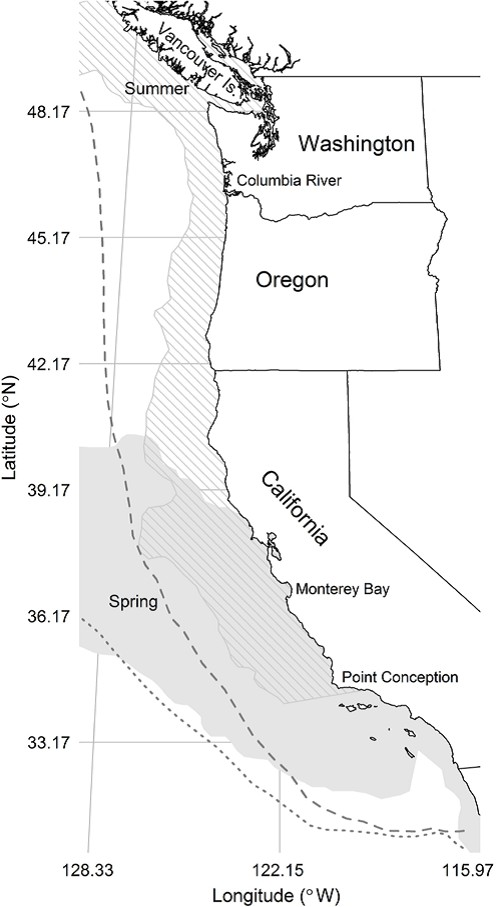
\includegraphics[width=\textwidth,height=6in]{content/images/clipboard-1472872065.png}

}

\subcaption{Sardine distribution}

\end{figure}%

\end{minipage}%
%
\begin{minipage}{0.50\linewidth}

\begin{figure}[H]

{\centering 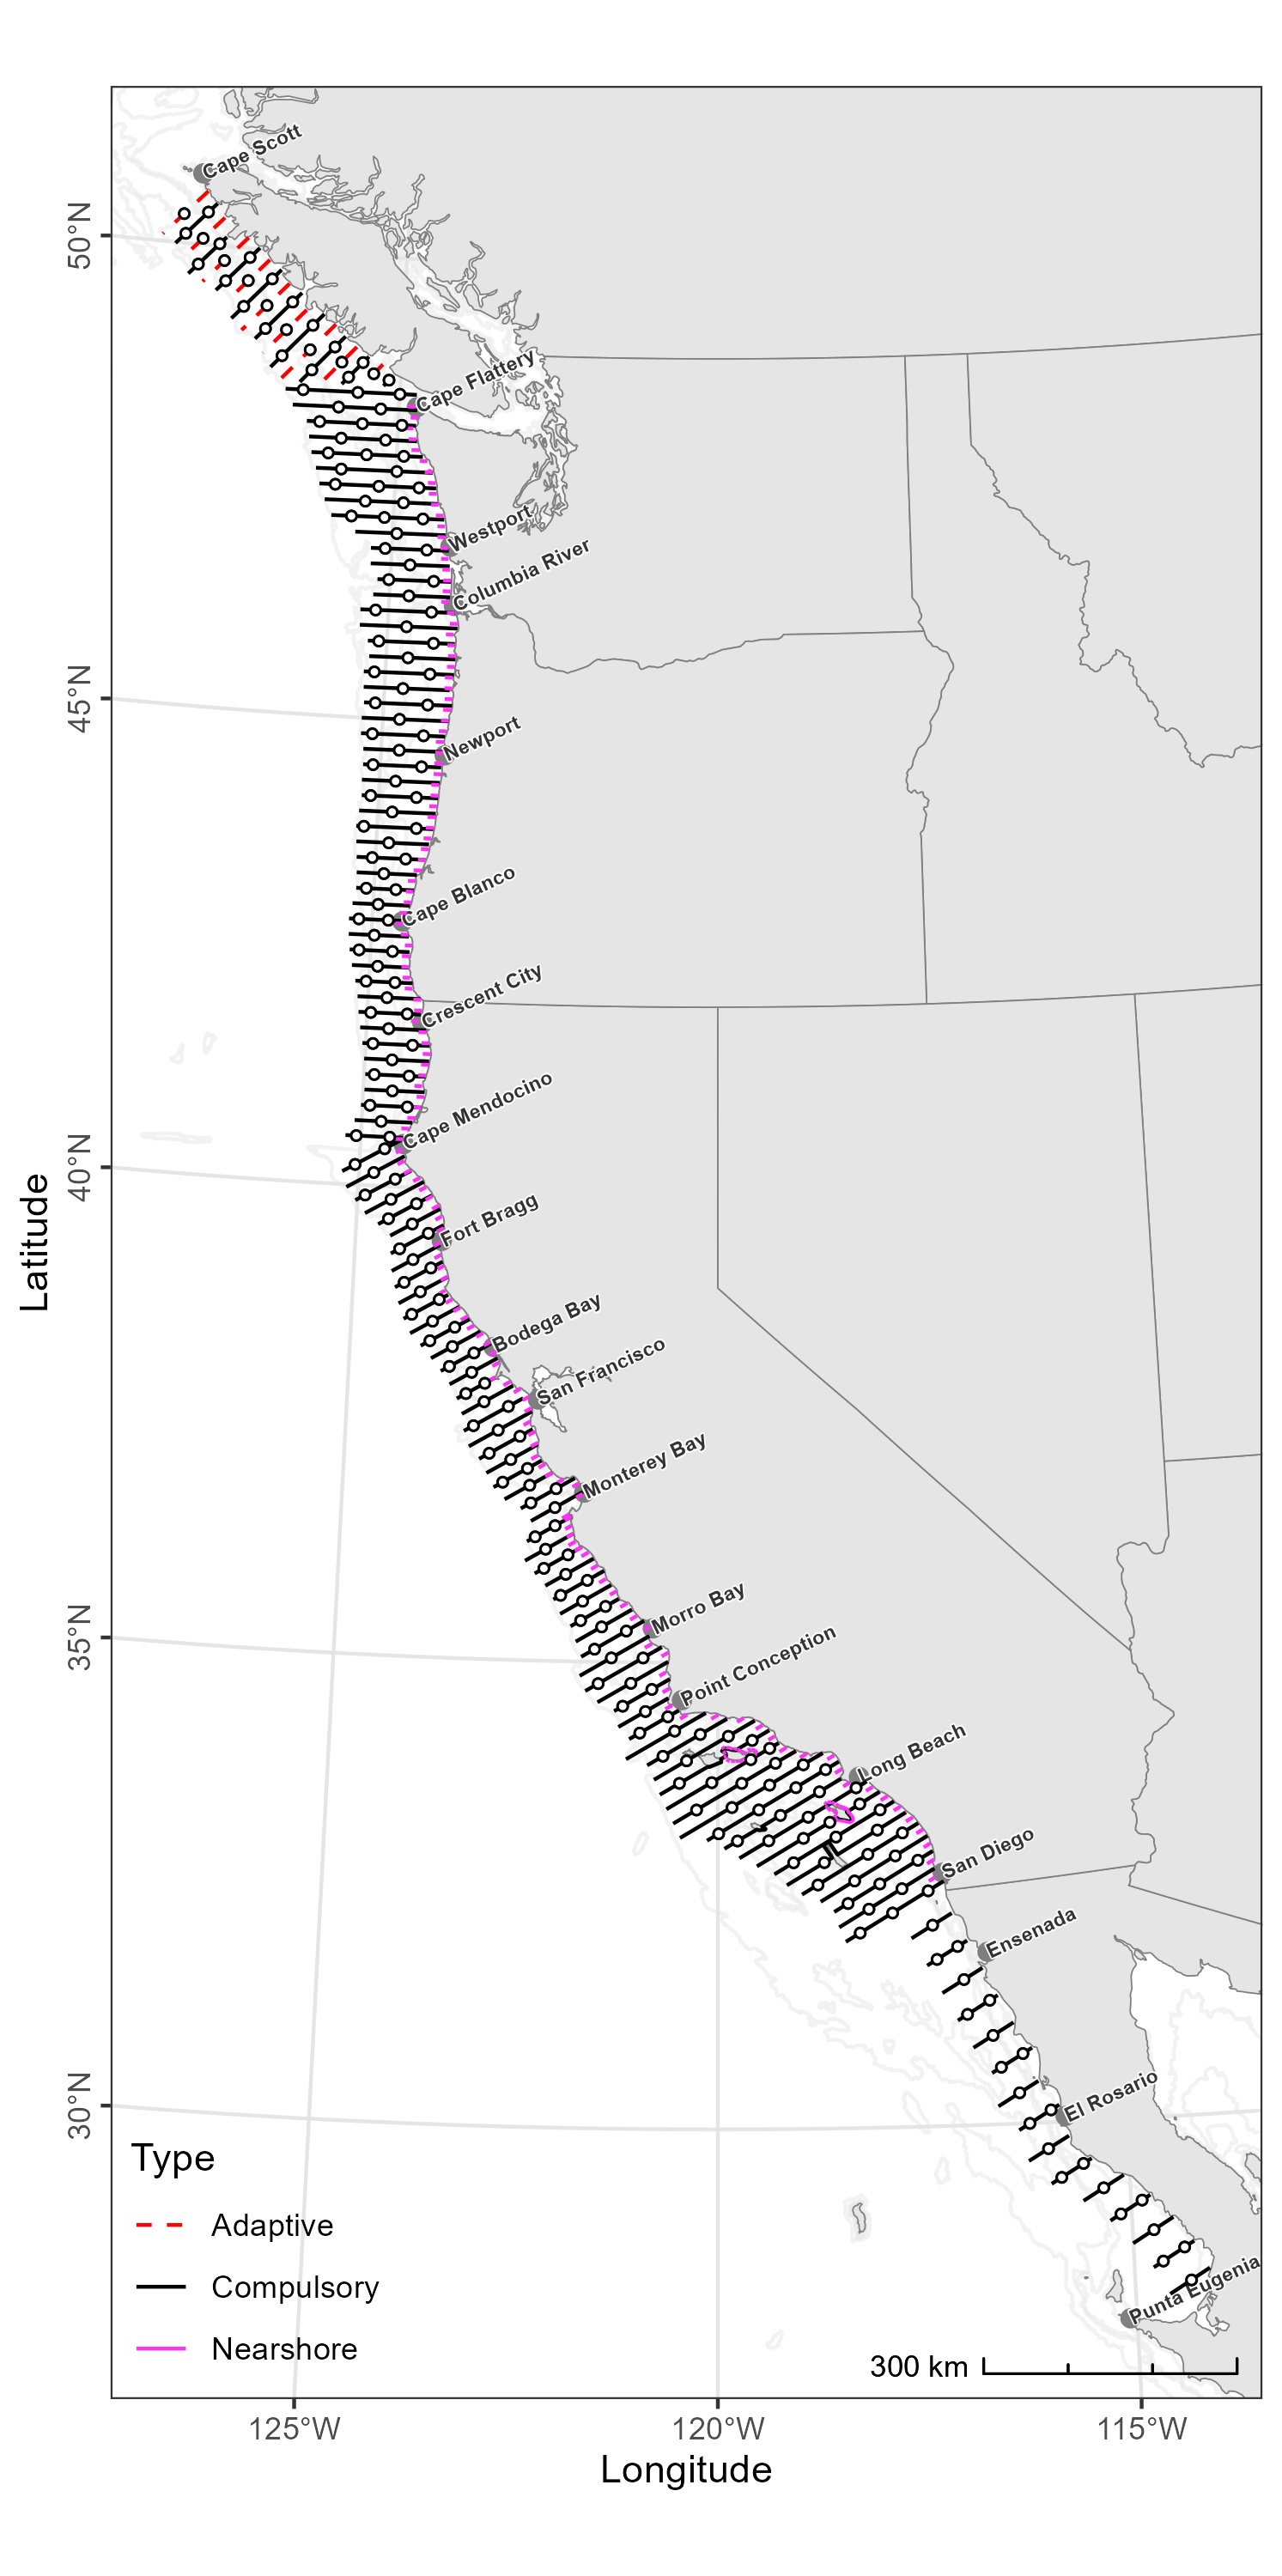
\includegraphics[width=\textwidth,height=6in]{content/images/fig_survey_map.png}

}

\subcaption{General sampling scheme}

\end{figure}%

\end{minipage}%

\caption{\label{fig-survey}On left, a conceptual spring (shaded region)
and summer (hashed region) distributions of potential habitat for the
northern stock of Pacific Sardine along the west coasts of Mexico, the
United States, and Canada. On right, the general sampling scheme of
planned core-region (solid black lines), adaptive (dashed red lines),
and nearshore lines (pink).}

\end{figure}%

\section{Research objectives:}\label{research-objectives}

\begin{enumerate}
\def\labelenumi{\arabic{enumi}.}
\tightlist
\item
  Acoustically map the distributions, measure the species compositions
  and size-frequency distributions, and estimate the abundances and
  biomasses of CPS present in the survey area, e.g., Pacific Sardine
  Sardinops sagax, Northern Anchovy (\emph{Engraulis mordax}), Pacifc
  Herring (\emph{Clupea pallasii}), Round Herring (\emph{Etrumeus
  acuminatus}), Pacific Mackerel (\emph{Scomber japonicus}), and Jack
  Mackerel (\emph{Trachurus symmetricus})
\item
  Characterize and investigate linkages to their biotic and abiotic
  environments
\item
  Gather information regarding their life histories
\item
  Compare the species composition and size distributions of trawls and
  near shore vessel purse seine sets.
\end{enumerate}

\section{Survey History:}\label{survey-history}

The SWFSC's ATM surveys of CPS in the CCE began in 2006 with a focus on
the northern stock of Pacific Sardine. Since then, they have expanded in
scope and objectives to include the larger forage-fsh assemblage and
krill. This evolution, and the migratory behavior of Pacific Sardine,
serve to explain the present survey region and design.

\section{Code of Conduct}\label{code-of-conduct}

\bookmarksetup{startatroot}

\chapter{Data Acquisition}\label{data-acquisition}

\section{Survey Equipment}\label{survey-equipment}

\subsection{Acoustic Instruments}\label{acoustic-instruments}

\begin{figure}[H]

{\centering 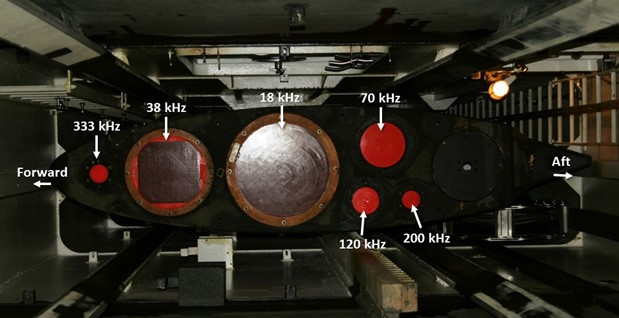
\includegraphics{content/images/transducers.jpg}

}

\caption{Transducer locations on the bottom of the centerboard aboard
Lasker.}

\end{figure}%

On \emph{Lasker} and \emph{Shimada}, multi-frequency Wideband
Transceivers (Simrad EK80 WBTs; Kongsberg) were confgured with
split-beam transducers (Simrad ES18, ES38-7, ES70-7C, ES120-7C,
ES200-7C, and ES333- 7C on \emph{Lasker} and ES18, ES38B, ES70-7C,
ES120-7C, and ES200-7C on \emph{Shimada}; Kongsberg). The transducers
were mounted on the bottom of a retractable keel or ``centerboard''. The
keel was retracted (transducers \textasciitilde5-m depth) during
calibration, and extended to the intermediate position (transducers
\textasciitilde7-m depth) during the survey. Exceptions were made during
shallow water operations, when the keel was re- tracted; or during times
of heavy weather, when the keel was extended (transducers
\textasciitilde9-m depth) to provide extra stability and reduce the
efect of weather-generated noise. Transducer position and motion were
measured at 5 Hz using an inertial motion unit (Applanix POS-MV;
Trimble).

\subsection{Underway CTD}\label{underway-ctd}

On \emph{Lasker} and \emph{Shimada}, conductivity and temperature
profiles were measured down to 300 m using calibrated sensors on a probe
cast from the vessel while underway (UnderwayCTD, or UCTD; Teledyne
Ocean- science). Casts were typically conducted between two to four
times along each transect. These data indicate the depth of the surface
mixed layer, above which most epipelagic CPS reside during the day.
These data were also used to estimate the time-averaged sound speed
(Demer, 2004), for estimating ranges to the sound scatterers, and
frequency-specifc sound absorption coefcients, for compensating signal
attenuation of the sound pulse between the transducer and scatterers
(Simmonds and MacLennan, 2005).

\section{Software}\label{software}

\subsection{Echosounder Software}\label{echosounder-software}

EK80

\subsection{NetTime}\label{nettime}

On \emph{Lasker} and \emph{Shimada}, the computer clocks were
synchronized with the GPS clock (UTC) using a synchronization software
called NetTime.

\subsection{EAL}\label{eal}

The 38-, 70-, 120-, 200-, and 333-kHz echosounders were controlled by
the EK80 Adaptive Logger
(EAL\href{file:///C:/Users/alice.beittel/Downloads/2024Renfree.docx\#_bookmark7}{2},
Renfree and Demer, 2016). The EAL optimizes the pulse interval based on
the seabed depth, while avoiding aliased seabed echoes, and was
programmed such that once an hour the echosounders would record three
pings in passive mode, for obtaining estimates of the background noise
level.

\subsection{K Sync}\label{k-sync}

To minimize acoustic interference on \emph{Lasker} and \emph{Shimada},
transmit pulses from the EK80s, acoustic Doppler current profler and
echosounder (Simrad-Kongsberg EC150-3C), multibeam echosounder (Simrad-
Kongsberg ME70), imaging sonar (Simrad-Kongsberg MS70), scanning sonar
(Simrad-Kongsberg SX90), and a separate acoustic Doppler current profler
(Teledyne RD Instruments OS75 ADCP) were triggered using a
synchronization system (Simrad K-Sync; Kongsberg). The K-Sync trigger
rate, and thus the echosounder ping interval, was modulated by the EAL
using the 18-kHz seabed depth provided by the Scientifc Computing System
(SCS).

\section{Raw Acoustic Data Format}\label{raw-acoustic-data-format}

Measurements of volume backscattering strength
(\emph{S\textsubscript{v}}; dB re 1 m2 m-3) and target strength
(\emph{TS}; dB re 1 m2), indexed by time and geographic positions
provided by GPS receivers, were stored in Simrad-Kongsberg .raw format
with a 1-GB maximum fle size. During daytime, the echosounders operated
in CW mode and logged to 60 m beyond the detected seabed range or to a
maximum range of 500, 500, 500, 300, and 150 m for 38, 70, 120, 200, and
333 kHz, respectively. During nighttime, the echosounders operated in FM
mode and logged to 100 m. For each acoustic instrument, the prefx for
each fle name is a concatenation of the survey name (e.g., 2307RL), the
operational mode (CW or FM), and the logging commencement date and time
from the EK80 software (v21.15.1). For example, a fle generated by the
Simrad-Kongsberg EK80 software for a WBT operated in CW mode is named
2307RL\_CW-D20220826-T155651.raw.

\bookmarksetup{startatroot}

\chapter{Data Workflow}\label{data-workflow}

\subsection{Data pipeline from boat to shore to
report}\label{data-pipeline-from-boat-to-shore-to-report}

\bookmarksetup{startatroot}

\chapter{Data Preparation}\label{data-preparation}

\subsection{Select regions of
interest}\label{select-regions-of-interest}

\subsubsection{Select data on transect
lines}\label{select-data-on-transect-lines}

\subsubsection{Integration stop and start
lines}\label{integration-stop-and-start-lines}

\bookmarksetup{startatroot}

\chapter{Data Processing}\label{data-processing}

Echoes from schooling CPS were identified using a semi-automated data
processing algorithm implemented using Echoview software (v13.1;
Echoview Software Pty Ltd). The filters and thresholds were based on a
subsample of echoes from randomly selected CPS schools. The aim of the
filter criteria is to retain at least 95\% of the noise-free backscatter
from CPS while rejecting at least 95\% of the non-CPS backscatter (Fig.
7). Data from Lasker, Shimada, Lisa Marie, and Long Beach Carnage were
processed using the following steps:

\begin{enumerate}
\def\labelenumi{\arabic{enumi}.}
\tightlist
\item
  Match geometry of all Sv variables to the 38-kHz Sv ;
\item
  Remove passive-mode pings;
\item
  Estimate and subtract background noise using the background noise
  removal function (De Robertis and Higginbottom, 2007) in Echoview
  (Figs. 7b, e);
\item
  Average the noise-free Sv echograms using non-overlapping 11-sample by
  3-ping bins;
\item
  Expand the averaged, noise-reduced Sv echograms with a 7 pixel x 7
  pixel dilation;
\item
  For each pixel, compute: Sv,200kHz − Sv,38kHz, Sv,120kHz − Sv,38kHz,
  and Sv,70kHz − Sv,38kHz;
\item
  Create a Boolean echogram for Sv differences in the CPS range: −13.85
  \textless{} Sv,70kHz − Sv,38kHz \textless{} 9.89 and − 13.5
  \textless{} Sv,120kHz − Sv,38kHz \textless{} 9.37 and − 13.51
  \textless{} Sv,200kHz − Sv,38kHz \textless{} 12.53;
\item
  For 120 and 200 kHz, compute the squared difference between the
  noise-filtered Sv (Step 3) and averaged Sv (Step 4), average the
  results using an 11-sample by 3-ping window to derive variance, then
  compute the square root to derive the 120- and 200-kHz standard
  deviations (σ120kHz and σ200kHz, respectively);
\item
  Expand the standard deviation echograms with a 7 pixel x 7 pixel
  dilation;
\item
  Create a Boolean echogram based on the standard deviations in the CPS
  range: σ120kHz \textgreater{} -65 dB and σ200kHz \textgreater{} -65
  dB. Diffuse backscattering layers have low σ (Zwolinski et al., 2010)
  whereas fsh schools have high σ;
\item
  Intersect the two Boolean echograms to create an echogram with
  ``TRUE'' samples for candidate CPS schools and ``FALSE'' elsewhere;
\item
  Mask the noise-reduced echograms using the CPS Boolean echogram (Figs.
  7c, f );
\item
  Create an integration-start line 5 m below the transducer
  (\textasciitilde10 m depth);
\item
  Create an integration-stop line 3 m above the estimated seabed (Demer
  et al., 2009), or to the maximum logging range (e.g., 350 m),
  whichever is shallowest;
\item
  Set the minimum Sv threshold to -60 dB (corresponding to a density of
  approximately three 20-cm-long Pacific Sardine per 100 m3);
\item
  Integrate the volume backscattering coefficients (sV , m2 m-3)
  attributed to CPS over 5-m depths and averaged over 100-m distances;
\item
  Output the resulting nautical area scattering coefficients (sA; m2
  nmi-2) and associated information from each transect and frequency to
  comma-delimited text (.csv) files.
\end{enumerate}

\bookmarksetup{startatroot}

\chapter{Figures and Tables}\label{figures-and-tables}

Markdown is a simple formatting syntax for authoring HTML, PDF, and MS
Word documents. For more details on using R Markdown see
\url{http://rmarkdown.rstudio.com}.

\section{Code}\label{code}

You can embed an R code chunk like this:

\begin{Shaded}
\begin{Highlighting}[]
\FunctionTok{summary}\NormalTok{(cars)}
\end{Highlighting}
\end{Shaded}

\begin{verbatim}
     speed           dist       
 Min.   : 4.0   Min.   :  2.00  
 1st Qu.:12.0   1st Qu.: 26.00  
 Median :15.0   Median : 36.00  
 Mean   :15.4   Mean   : 42.98  
 3rd Qu.:19.0   3rd Qu.: 56.00  
 Max.   :25.0   Max.   :120.00  
\end{verbatim}

\section{Including Plots}\label{including-plots}

You can also embed plots and reference them, like so
Figure~\ref{fig-pressure}.

\begin{figure}

\centering{

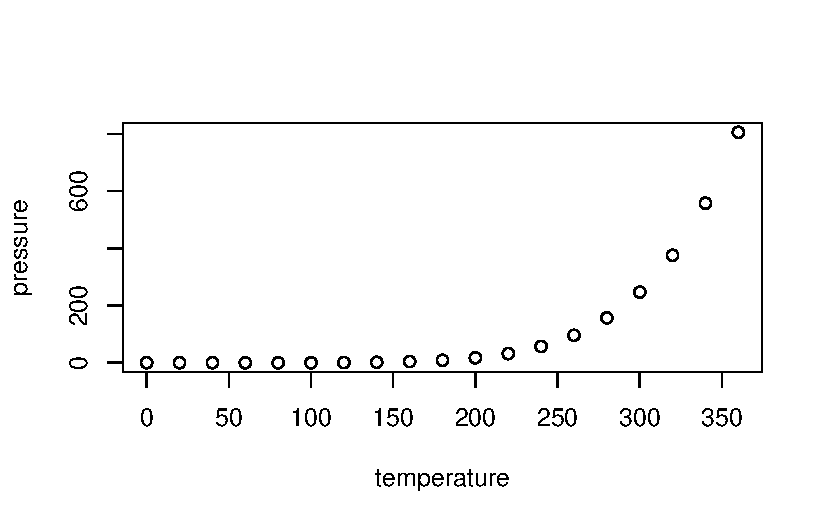
\includegraphics{content/figures_and_tables_files/figure-pdf/fig-pressure-1.pdf}

}

\caption{\label{fig-pressure}Plot of pressure}

\end{figure}%

Note that the \texttt{echo\ =\ FALSE} parameter was added to the code
chunk to prevent printing of the R code that generated the plot.

\section{Including Tables}\label{including-tables}

You can also embed tables and reference them with Table~\ref{tbl-iris}.

\begin{Shaded}
\begin{Highlighting}[]
\FunctionTok{library}\NormalTok{(knitr)}
\FunctionTok{kable}\NormalTok{(}\FunctionTok{head}\NormalTok{(iris))}
\end{Highlighting}
\end{Shaded}

\begin{longtable}[]{@{}rrrrl@{}}

\caption{\label{tbl-iris}Iris Data}

\tabularnewline

\toprule\noalign{}
Sepal.Length & Sepal.Width & Petal.Length & Petal.Width & Species \\
\midrule\noalign{}
\endhead
\bottomrule\noalign{}
\endlastfoot
5.1 & 3.5 & 1.4 & 0.2 & setosa \\
4.9 & 3.0 & 1.4 & 0.2 & setosa \\
4.7 & 3.2 & 1.3 & 0.2 & setosa \\
4.6 & 3.1 & 1.5 & 0.2 & setosa \\
5.0 & 3.6 & 1.4 & 0.2 & setosa \\
5.4 & 3.9 & 1.7 & 0.4 & setosa \\

\end{longtable}

\bookmarksetup{startatroot}

\chapter{Rendering with Code}\label{rendering-with-code}

You can have code (R, Python or Julia) in your qmd file. You will need
to have these installed on your local computer, but presumably you do
already if you are adding code to your qmd files.

\begin{Shaded}
\begin{Highlighting}[]
\NormalTok{x }\OtherTok{\textless{}{-}} \FunctionTok{c}\NormalTok{(}\DecValTok{5}\NormalTok{, }\DecValTok{15}\NormalTok{, }\DecValTok{25}\NormalTok{, }\DecValTok{35}\NormalTok{, }\DecValTok{45}\NormalTok{, }\DecValTok{55}\NormalTok{)}
\NormalTok{y }\OtherTok{\textless{}{-}} \FunctionTok{c}\NormalTok{(}\DecValTok{5}\NormalTok{, }\DecValTok{20}\NormalTok{, }\DecValTok{14}\NormalTok{, }\DecValTok{32}\NormalTok{, }\DecValTok{22}\NormalTok{, }\DecValTok{38}\NormalTok{)}
\FunctionTok{lm}\NormalTok{(x }\SpecialCharTok{\textasciitilde{}}\NormalTok{ y)}
\end{Highlighting}
\end{Shaded}

\begin{verbatim}

Call:
lm(formula = x ~ y)

Coefficients:
(Intercept)            y  
      1.056        1.326  
\end{verbatim}

\section{Modify the GitHub Action}\label{modify-the-github-action}

You will need to change the GitHub Action in \texttt{.github/workflows}
to install these and any needed packages in order for GitHub to be able
to render your webpage. The GitHub Action install R since I used that in
\texttt{code.qmd}. If you use Python or Julia instead, then you will
need to update the GitHub Action to install those.

If getting the GitHub Action to work is too much hassle (and that
definitely happens), you can alway render locally and publish to the
\texttt{gh-pages} branch. If you do this, make sure to delete or rename
the GitHub Action to something like

\begin{verbatim}
render-and-publish.old_yml
\end{verbatim}

so GitHub does not keep trying to run it. Nothing bad will happen if you
don't do this, but if you are not using the action (because it keeps
failing), then you don't need GitHub to run it.

\section{Render locally and publish to gh-pages
branch}\label{render-locally-and-publish-to-gh-pages-branch}

To render locally and push up to the \texttt{gh-pages} branch, open a
terminal window and then \texttt{cd} to the directory with the Quarto
project. Type this in the terminal:

\begin{verbatim}
quarto render gh-pages
\end{verbatim}

\bookmarksetup{startatroot}

\chapter{References}\label{references}

Quarto has powerful references functionality. You can easily insert
citations from Zotero libraries that you maintain in the cloud (on
Zotero). This allows the whole team to update the library and you can
sync up to that library. Read about this on the Quarto documentation on
\href{https://quarto.org/docs/visual-editor/technical.html\#citations}{citations}.
Google youtube videos on this also to see it in action.

Add a \texttt{.bib} file in to your project or add a linked Zotero
library via RStudio in Visual mode with Tools \textgreater{} Project
Options\ldots{} \textgreater{} R Markdown \textgreater{} select custom
libraries from the Zotero dropdown.

The you can type \texttt{@} and you will see a dropdown of the
references in your libraries. You can then select the ones to add. If
you don't see the one you need, you can paste in the DOI and it will be
added to your references file (with all the info). The references will
be added to your references section of your book automatically.

See the \texttt{references.qmd} file for how to include the references.

\begin{itemize}
\item
  \texttt{@ansley1981} will produce Ansley and Davis (1981)
\item
  \texttt{{[}@ansley1981{]}} will produce (Ansley and Davis 1981).
\end{itemize}

\bookmarksetup{startatroot}

\chapter*{References}\label{references-1}
\addcontentsline{toc}{chapter}{References}

\markboth{References}{References}

\phantomsection\label{refs}
\begin{CSLReferences}{1}{0}
\bibitem[\citeproctext]{ref-ansley1981}
Ansley, H. L. H., and C. D. Davis. 1981. {``Migration and Standing Stock
of Fishes Associated with Artificial and Natural Reefs on Georgia{'}s
Outer Continental Shelf.''} Brunswick, Georgia, USA.

\end{CSLReferences}


\backmatter

\end{document}
